\section{Projektstrukturplan}

\subsection{5. Semester}

hier auf alten psp als beigefügte Datei verweisen (bitte text aus word übertragen). Wer dieses Kapitel schreibt bitte nach abschluss unbedingt Rücksprache mit Sebbel halten um sicher zu stellen, dass die datei auch wirklich angehängt wird!!!!!

\subsection{6. Semester}

Hier entweder 3 unterkapitel für die einzelnen Teilprojekte (captive Portal, lunchapp, research) udn einen gesamt psp mit Teammeetings oder nur den Überblick und die detail aspekte (z.b. Arbeitspakete für Lunchapp) in die jeweilige Abschnitte in Kapitel 4. Bitte Rücksprache mit Sebbel über genaues vorgehen BEVOR der abschnitt 6. Semester erstellt wird!


\subsection{Kanbanboard}

Nach der Erstellung des \gls{psp} wurde daraus innerhalb der Webanwendung Trello ein Kanbanboard erstellt (siehe \ref{fig:frame:kanban}). In diesem Kanbanboard werden jedem Arbeitspaket die verantwortlichen Personen, die benötigten Dateien, der Bearbeitungszeitraum und auch der Bearbeitungsstatus zugeordnet werden. Hierdurch ist der Fortschritt des Projekts und die zu bearbeitenden Aufgaben für alle Mitglieder einsehbar. Durch die Möglichkeit, Kommentare zu einzelnen Arbeitspaketen hinzuzufügen, kann direktes Feedback für Aufgaben anderer Teammitglieder gegeben werden und die gebrauchte Arbeitszeit eingetragen werden. Die gezielte Nutzung dieser Möglichkeit vereinfachte das Projektmanagement erheblich.

\begin{figure}[H]
\centering
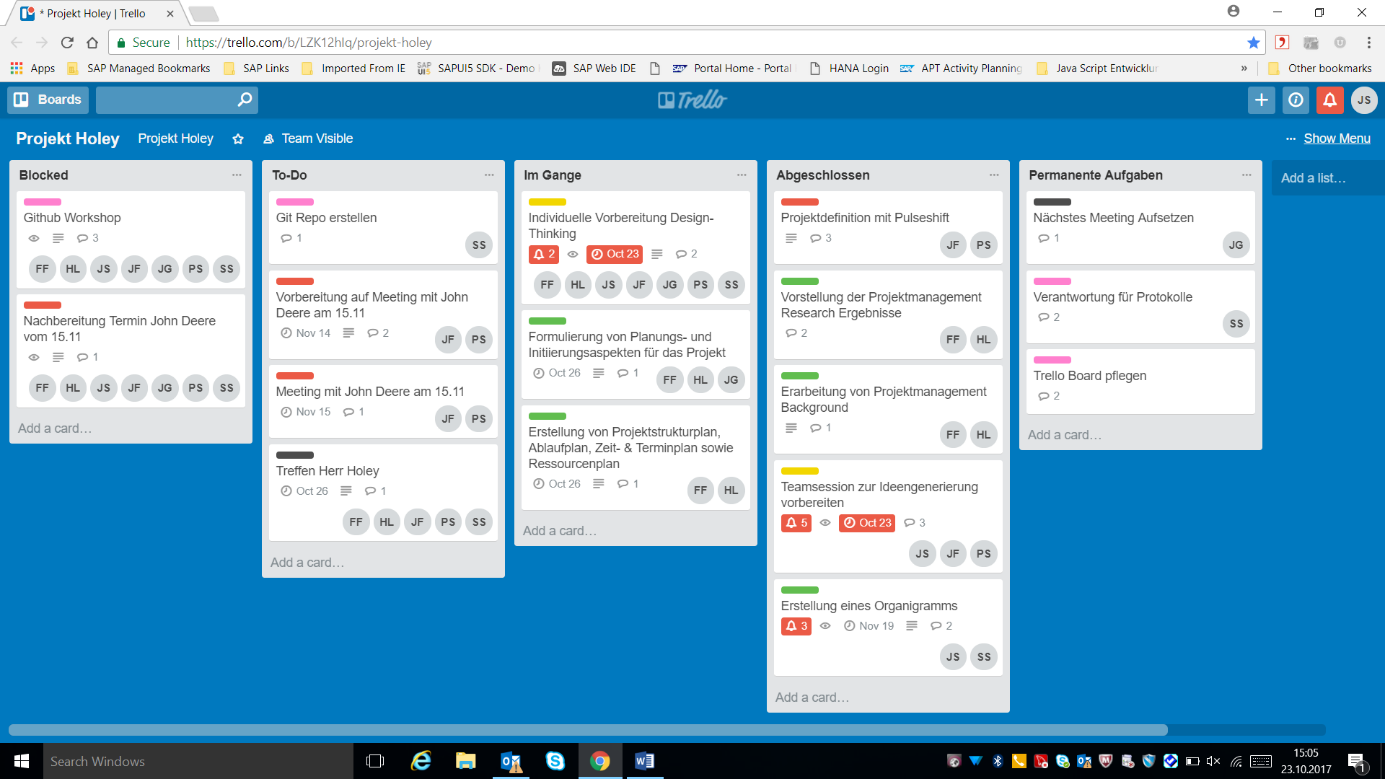
\includegraphics[width=1\textwidth]{images/trello}
\caption[Bildschirmabgriff des Kanbanboards in Trello]{Bildschirmabgriff des Kanbanboards in Trello}
\label{fig:frame:kanban}
\end{figure}
